

\section{Offline Schema Study Details}\label{supp:study_details}


All experiments for the design choice study, unless specified, use the same configuration as \base. For mixing over the DCLM topics, we constructed a sparse swarm of size $K = 128$.
We also mix at the source level over DCLM, Stack-Edu, ArXiv, FineMath 3+, olmOCR Science PDFs, Wikipedia, and Pes2o (see Table~\ref{tab:domain_sizes}). For the sources, we constructed a dense swarm of size $K = 64$. We use log-linear regression per task, an exact solver with $\lambda = 0.05$, and enforced repetition constraints in the optimization problem with $R =$ 6T and $k = 4$.


\subsection{RQ1: Proxy model size} 

\textbf{Details.} Table~\ref{tab:model_architectures} contains details about the architectures of the 1M, 15M, 30M, and 60M proxy models we train. 

\begin{table}[htb]
\centering
\caption{Proxy Model Architecture Configurations.}
\label{tab:model_architectures}
\begin{tabular}{lcccc}
\toprule
\textbf{Parameter} & \textbf{1M} & \textbf{15M} & \textbf{30M} & \textbf{60M} \\
\midrule
Vocab size & 100,352 & 100,352 & 100,352 & 100,352 \\
\texttt{n\_layers} & 4 & 8 & 4 & 8 \\
\texttt{n\_heads} & 4 & 4 & 8 & 8 \\
\texttt{d\_model} & 16 & 128 & 256 & 384 \\
\texttt{head\_dim} & 4 & 32 & 32 & 48 \\
\bottomrule
\end{tabular}
\end{table}


\subsection{RQ2: Swarm size} 

\textbf{Additional results.} In Figure~\ref{fig:swarm_size_1B}, we vary $K = c(m+1)$ for $c = 1, 2, 3, 4$ and $m=6, 24$ and study its effect on downstream BPB of 1B models. Despite having fewer $m$, the error curves when scaled according to $c$ collapse together, suggesting that the $\mathcal{O}(m)$ sample complexity holds at both 30M and 1B model scales. 

\textbf{Details.} For the results in Figure~\ref{fig:swarm_size} and Figure~\ref{fig:swarm_size_1B}, we constructed proposed mixes using a search-based solver rather than an exact solver. We also did not enforce repetition constraints and had originally included 5 additional metrics in our evaluation suite: Qasper Yes/No, Sciriff Yes/No, LabBench DBQA, LabBench ProtocolQA, and MedQA EN. 

For $m=24$, we used all WebOrganizer DCLM topics. For $m < 24$, we selected the $m$ largest domains. In particular, for $m=18$, we used: Art and Design, Crime and Law, Education and Jobs, Electronics and Hardware, Entertainment, Finance and Business, Games, Health, Literature, Politics, Religion, Science Math and Technology, Social Life, Software, Software Development, Sports and Fitness, Transportation, Travel and Tourism. 
For $m=12$, we used: Crime and Law, Education and Jobs, Entertainment, Finance and Business, Games, Health, Literature, Politics, Religion, Science Math and Technology, Software, and Software Development.
For $m=6$, we used: Entertainment, Finance and Business, Games, Health, Politics, and Science Math and Technology.


\begin{figure}
    \centering
    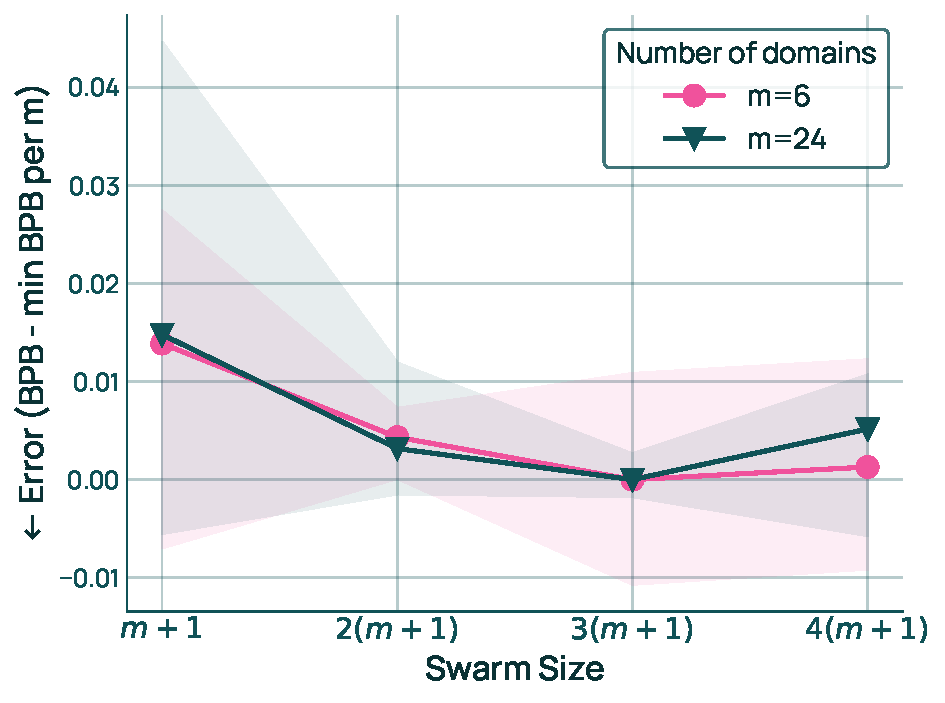
\includegraphics[width=0.48\linewidth]{figs/contribution_1/log_linear_sample_complexity_1B.pdf}
    \caption{Error on 1B models versus swarm size. Similar to Figure~\ref{fig:swarm_size}, we see that the error curves collapse across both $m$, supporting our finding that $K$ needs $\mathcal{O}(m)$ runs to obtain strong downstream performance. Results are averaged across 3 random seeds, and the intervals indicate min and max results.}
    \label{fig:swarm_size_1B}
\end{figure}


\subsection{RQ3: Swarm distribution}\label{supp:swarm_distribution}

\textbf{Details.} To construct the sparse and dense swarms, we first generated mixes sampled from a Dirichlet distribution.
For the dense swarm, we discarded any mixes that have domains with 0 weight, and for the sparse swarm, we enforced that if the weight of a domain is less than 0.05, then it is clipped to 0. The entire mixture is normalized afterwards. 

For the centering experiments, we compared a swarm with a natural Dirichlet prior to a strong and weak prior. The strong prior was the proposed mix obtained using the natural swarm. The weak prior was a mix that aimed to maximize BPB using the the natural swarm using a simulation-based solver. Regardless of the choice of Dirichlet prior, we used the natural distribution in the KL regularization term of the objective for fair comparison.

For both sets of experiments, we constructed a held-out test set containing of 30 samples, where 15 were from a Dirichlet distribution centered around the sparse swarm's optimal mix and 15 were from a Dirichlet distribution centered around the dense swarm's optimal mix. This measures regression fit in high-performance regions of the mixture space, which matters in the mixture optimization step. 

\subsection{RQ4: Regression model family}\label{supp:regression}

\textbf{Additional results.} Figure~\ref{fig:regression_models_olmo3} compares the downstream performance and regression fit (measured on three random train-test splits of the swarm, each with 10 test mixes) across several regression model families at the source level. Across both metrics, we see that the log-linear regression model outperforms other approaches. 

In Figure~\ref{fig:k_vs_m_dclm}, we plot the relationship between swarm size, number of domains, and regression fit across all regression model families over DCLM topics. These figures reveal that different regression model families have different sample complexity and regimes in which they do well. This offers a potential explanation for why existing methods lack consensus. 

\begin{figure}
    \centering
    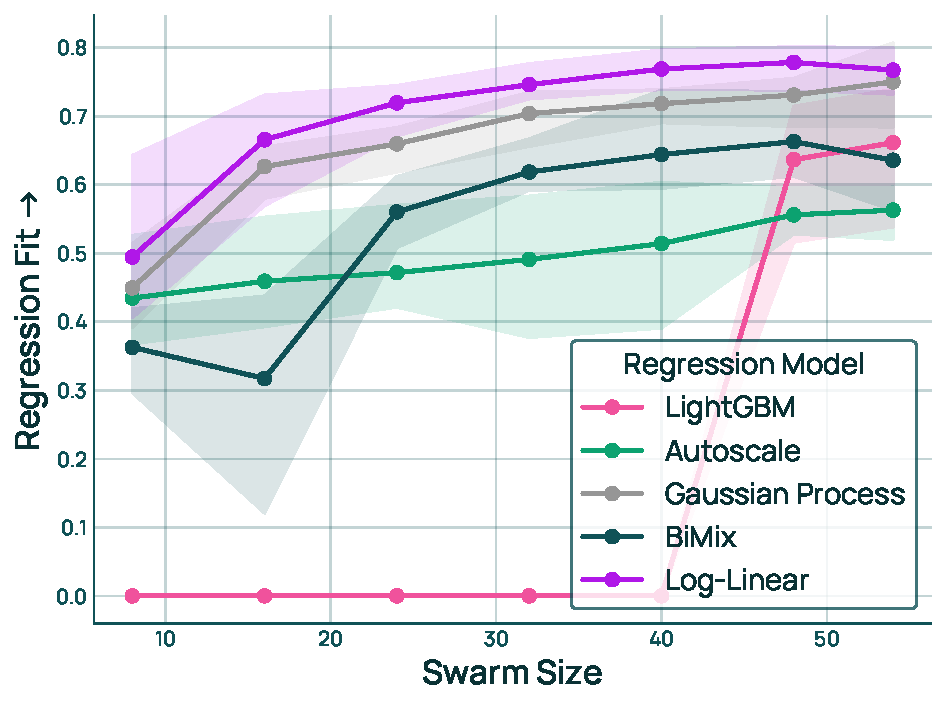
\includegraphics[width=0.5\linewidth]{figs/contribution_1/regression_models_vs_K_vs_m_olmo3.pdf}
    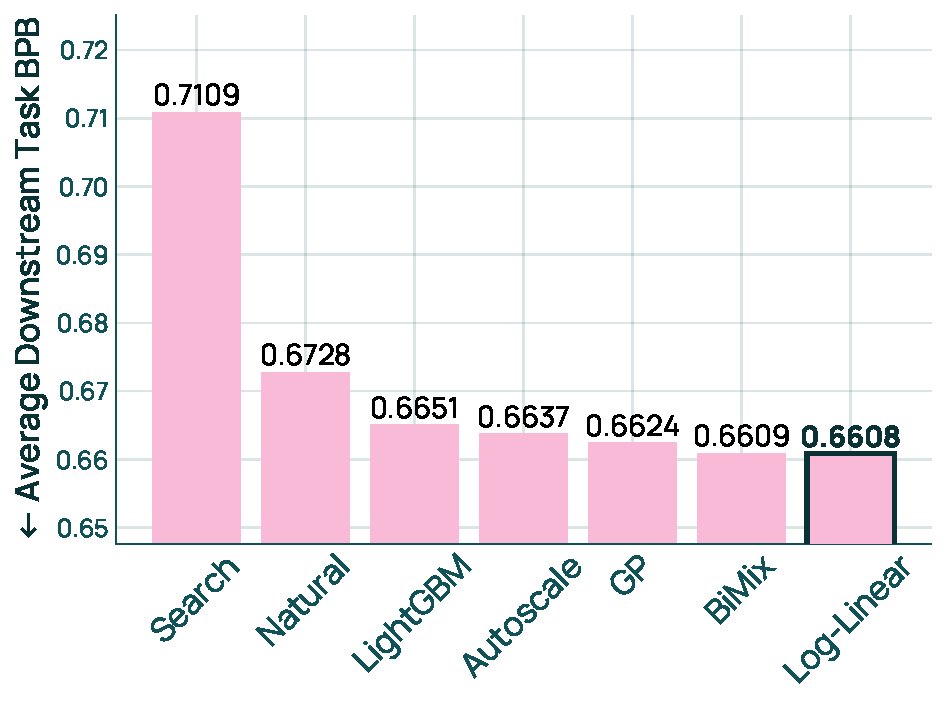
\includegraphics[width=0.48\linewidth]{figs/contribution_1/regression_models_performance_olmo3.pdf}
    \caption{Left: Regression fit versus swarm size across regression models when mixing across sources. Results are averaged across 3 random seeds, and the intervals indicate min and max results. Right: downstream performance of regression models over sources.}
    \label{fig:regression_models_olmo3}
\end{figure}


\begin{figure}
    \centering
    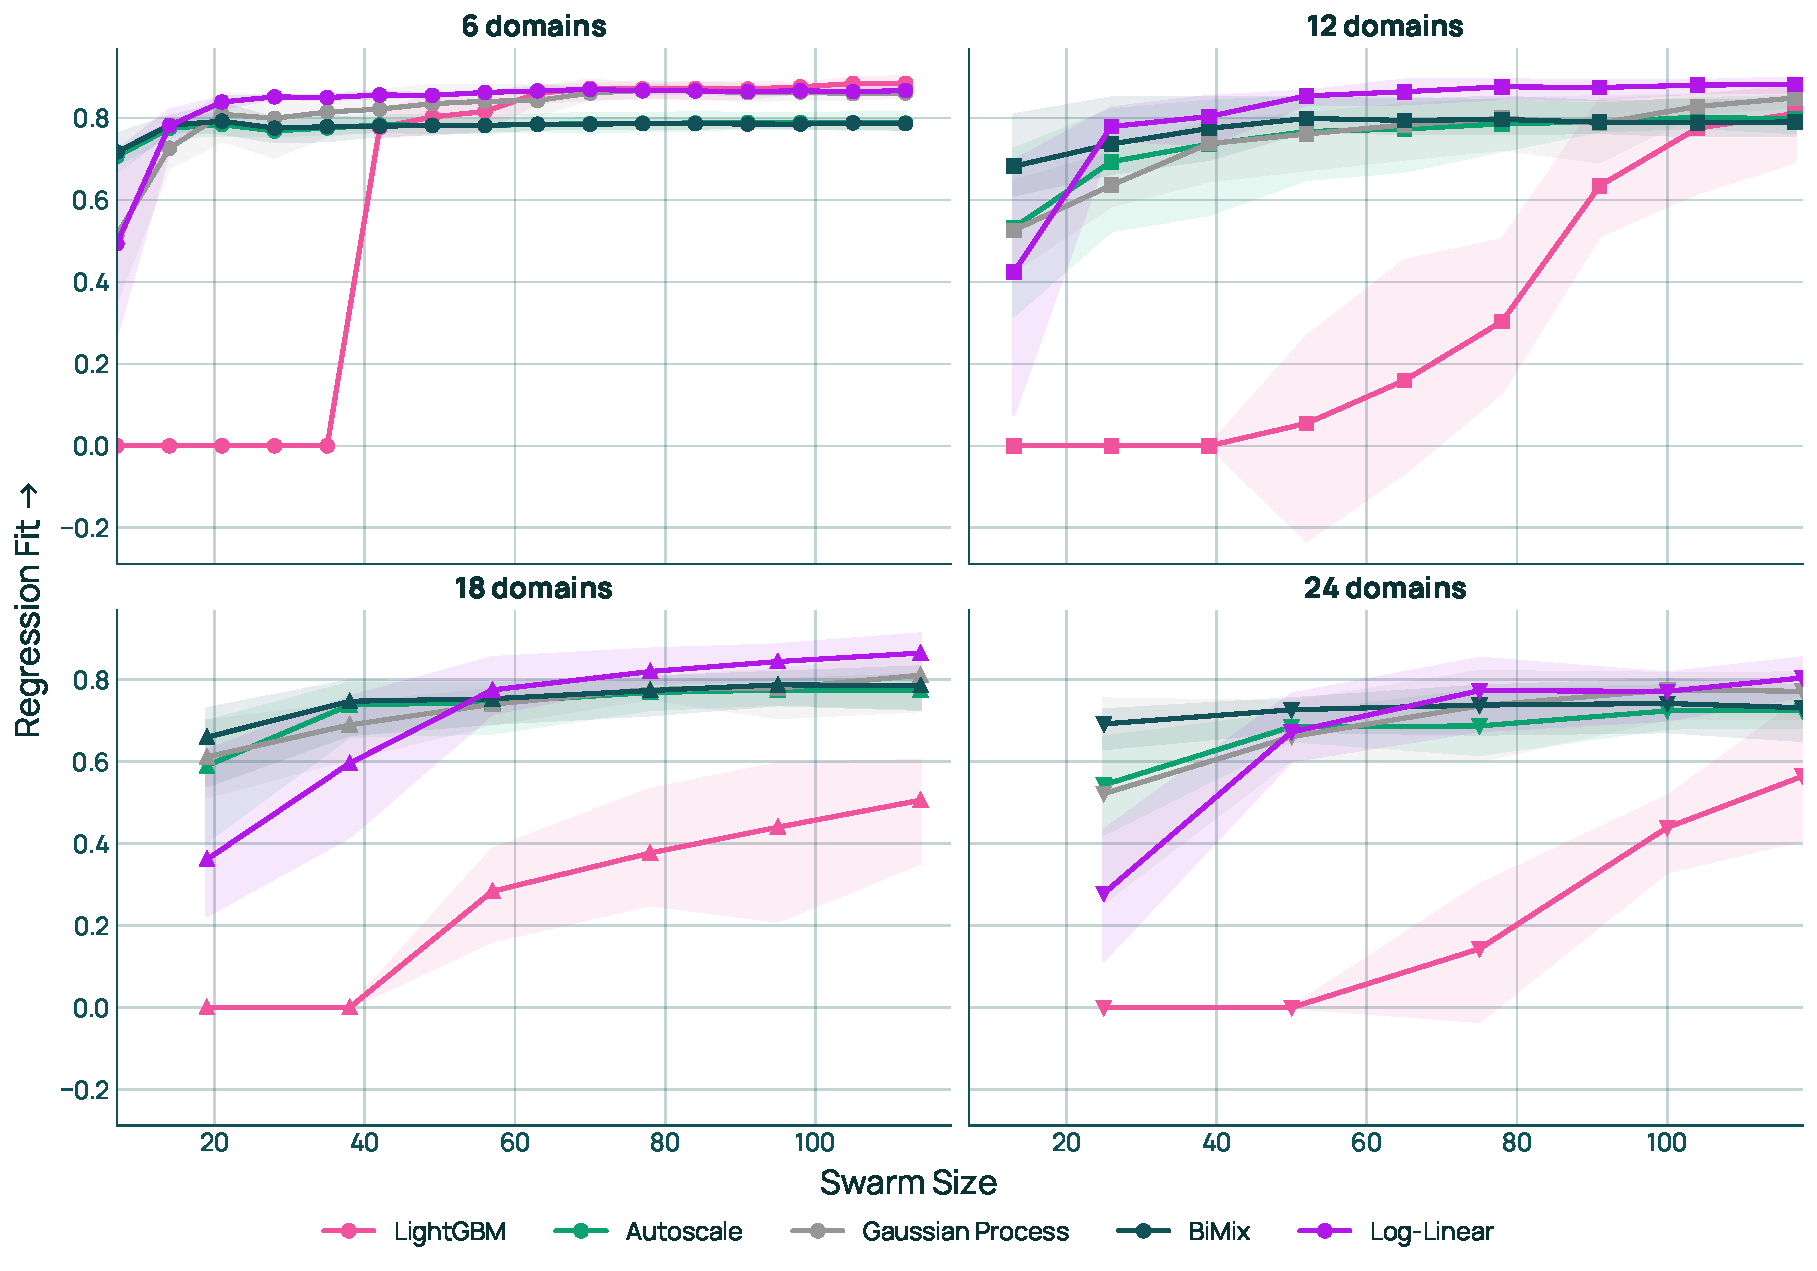
\includegraphics[width=\linewidth]{figs/contribution_1/regression_models_vs_K_vs_m_dclm.pdf}
    \caption{Regression fit versus swarm size and number of domains across regression models when mixing on DCLM topics. Across $m=6, 12, 18, 24$ domains, each regression model requires different swarm sizes to obtain good regression fit. Results are averaged across 3 random seeds, and the intervals indicate min and max results.}
    \label{fig:k_vs_m_dclm}
\end{figure}



\textbf{Details.} We describe how we adapt the regression models from BiMix~\citep{ge2025bimixbivariatedatamixing}, Autoscale~\citep{kang2025autoscalescaleawaredatamixing}, and Data Mixing Laws~\citep{ye2025datamixinglawsoptimizing} to our setting where performance is measured on a set of downstream tasks.

\begin{itemize}
    \item BiMix: The BiMix mixing law models the validation loss on domain $i$ as a function of the mixture ratio on domain $i$ and the number of training steps $s$:
    \begin{align}
        \hat{f}_i(p, s) = \frac{A_i}{p_i^{\alpha_i}} \bigg( \frac{B_i}{s^{\beta_i}} + C_i\bigg) \; \forall i \in [m].
    \end{align}

    Since we do not model the number of steps and instead directly transfer the proposed mix from the proxy scale to the target scale, this mixing law simplifies to $\hat{f}_i(p) = A_i p_i^{-\alpha_i}$, where the constants are absorbed into $A_i$. To extend this mixing law to downstream tasks rather than validation loss on training domains, we assume that task BPB can be modeled as a weighted average of training domain-specific mixing laws. Therefore, for each downstream task $i$, the BiMix mixing law for our setting is:
    \begin{align}
        \hat{f}_i(p) = \sum_{j = 1}^m A_{ij} p_j^{-\alpha_{ij}}.
    \end{align}

    \item AutoScale: The AutoScale mixing law models validation loss on a held-out dataset $i$ as a function of the mixture and the number of tokens $R$:
    \begin{align}
        \hat{f}(p, R) = \sum_{j = 1}^m \bigg((N^{j}_0 + p_j R)^{-\gamma_{j}} + l_j\bigg),
     \end{align}

     where $N^j_0$ is the ``effective'' number of tokens of all other domains excluding $j$.
     The original paper fits separate parameters for each domain using perturbed runs; we instead fit all parameters jointly using our larger swarm. We make two modifications. First, we replace the per-domain constants $l_j$ with a single constant term $c_i$ corresponding to a given task $i$. Second, instead of directly learning $N^j_0$, which can be quite large given the order of magnitude of $R$, we rewrite $N^j_0 + p_j R$ as $R(A_{ij} + p_j)$ and learn $A_{ij}$. Therefore, for each downstream task $i$, the AutoScale mixing law for our setting is:
     \begin{align}
         \hat{f}_i(p) = c_i + \sum_{j = 1}^m (R(   A_{ij} + p_j))^{-\alpha_{ij}}.
     \end{align}

     \item Data Mixing Laws: The mixing law models the validation loss on domain $i$ as:
     \begin{align}
         \hat{f}_i(p) = c_i + k_i \exp\bigg(\sum_{j = 1}^m t_{ij} p_j\bigg).\label{eq:dml_original}
     \end{align}

     The paper also extends this to out-of-domain validation sets by expressing them as a linear combination of training domains, namely $\hat{f}(p) = \sum_{i = 1}^m s_i \Big(c_i + k_i \exp \big(\sum_{j = 1}^m t_{ij} p_j\big) \Big)$. We use the first, simpler form~\eqref{eq:dml_original} directly for downstream tasks, treating each task's performance as a function of the mixture on training domains. Moreover, we observe that $k_i$ can be absorbed into the linear term; rewriting \eqref{eq:dml_original} as $c_i + \exp(\sum_{j = 1}^m t_{ij} p_j + \log k_i)$ shows that $k_i$ acts as an intercept term.  Since $p$ sums up to $1$, this intercept is redundant and can be dropped. Therefore, our final log-linear mixing law is
     \begin{align}
         \hat{f}_i(p) = c_i + \exp\bigg(\sum_{j = 1}^m A_{ij} p_j\bigg). \label{eq:app_log_linear}
     \end{align}
     
    \end{itemize}


Next, we provide implementation details for each model:
\begin{itemize}
    \item Search: we select the swarm run that has the best average BPB and satisfies the data repetition constraints.
    \item LightGBM: we use the hyperparameters from RegMix~\citep{liu2025regmixdatamixtureregression}. However, we did not use an evaluation set for early stopping, since we noticed that RegMix used the same set of mixes for early stopping and for reporting performance. We solve the optimization problem using search, as is done in RegMix.
    \item Gaussian Process: we use scikit-learn's GaussianProcessRegressor. We solve the optimization problem using search, as is done in~\citet{chen2025admirebayesoptaccelerateddatamixture}.
    \item BiMix: we use SciPy least squares to fit the regression models. We solve the optimization problem using search, an exact solver, and exact solver with KL regularization ($\lambda = 0.05$) in Table~\ref{tab:bimix_autoscale_solvers}. Based on the results, we decided to use a search-based solver when evaluating BiMix.
    \item AutoScale: we use SciPy least squares to fit the regression models. We solve the optimization problem using search, an exact solver, and exact solver with KL regularization ($\lambda = 0.05$)in Table~\ref{tab:bimix_autoscale_solvers}. Based on the results, we decide to use an exact solver when evaluating Autoscale.
    \item Log-linear: we use the fitting code from~\citet{ye2025datamixinglawsoptimizing}. We solve the optimization problem using CVXPY, while results for other solvers are discussed in \S\ref{sec:optimization}.
\end{itemize}

\begin{table}[t]
\centering
\small
\caption{Downstream performance of BiMix and AutoScale regression models on DCLM topics using exact optimization, exact + KL regularization ($\lambda = 0.05$), and search. Based on these findings, we use an exact solver with Autoscale and a search-based solver for BiMix for the rest of our study.}
\begin{tabular}{lccc}
\toprule
\textbf{Method} & \textbf{Exact (0.0)} & \textbf{Exact + KL (0.05)} & \textbf{Search} \\
\midrule
BiMix      & 0.776733 & 0.790188 & \textbf{0.768153} \\
Autoscale  & \textbf{0.798084} & 0.804814 & 0.808775 \\
\bottomrule
\end{tabular}
\label{tab:bimix_autoscale_solvers}
\end{table}





\subsection{RQ5: Regression granularity}

\textbf{Additional results.} Figure~\ref{fig:regression_granularity_30m} shows the performance of various regression granularities at the 30M scale. While the downstream BPB results at the 1B scale (Table~\ref{tab:granularity}) demonstrates that per-family performs the worst, the 30M performance results are in line with the regression fits of each granularity; per-task performs the best, followed by per-family and aggregated. 


\begin{figure}
    \centering
    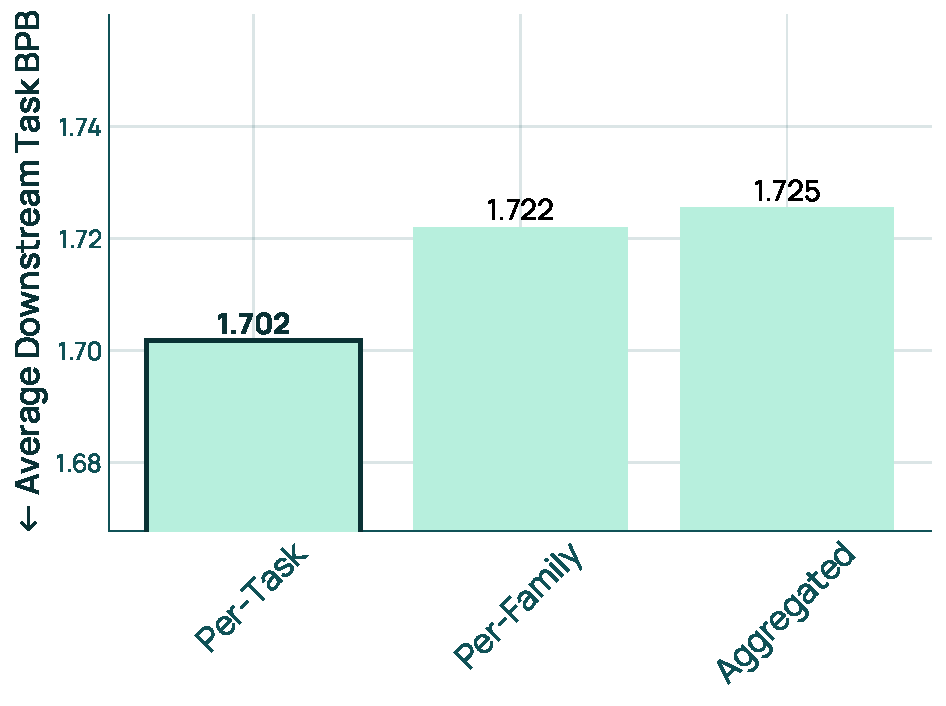
\includegraphics[width=0.5\linewidth]{figs/contribution_1/regression_granularity_30m.pdf}
    \caption{30M performance across regression granularities. The performance is monotonic in the task granularity, matching with the regression fit findings from Table~\ref{tab:granularity}.}
    \label{fig:regression_granularity_30m}
\end{figure}


\textbf{Details.} The task families we used are defined in Table~\ref{tab:eval_suite}: Math, Code, and QA. We constructed a held-out test set containing of 45 samples, consisting of 15 samples from a Dirichlet distribution centered around each regression granularity's respective proposed mix.
This measures regression fit in high-performance regions of the mixture space, which matters in the mixture optimization step. 


\subsection{RQ6: Data repetition constraints}

\textbf{Additional results.} Figure~\ref{fig:vary_repetition_factor} is the full version of Figure~\ref{fig:vary_rep_top_7}, showing the weights over all $24$ DCLM topics when we vary the repetition factor $k$.


\begin{figure}
    \centering
    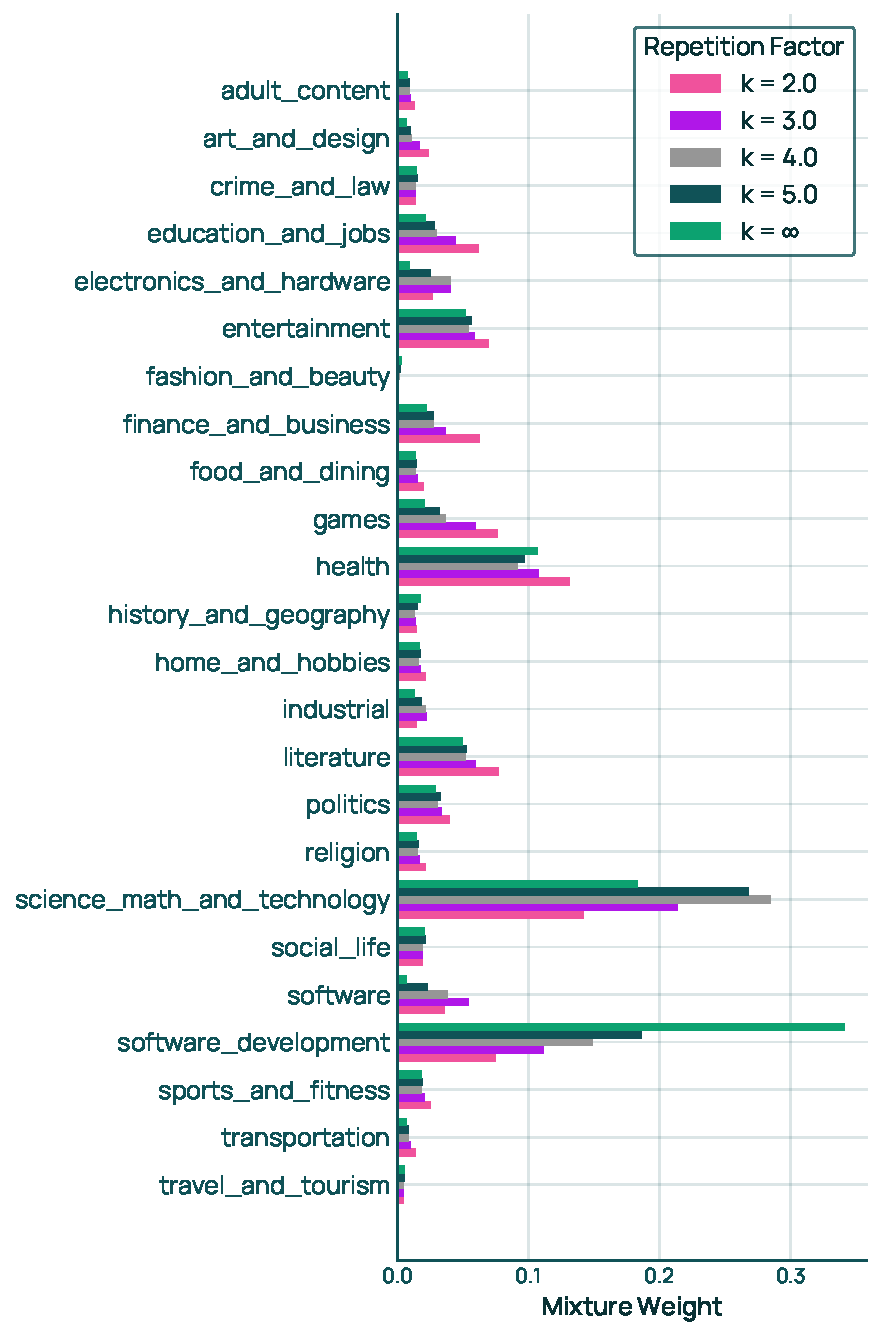
\includegraphics[width=0.6\linewidth]{figs/contribution_1/vary_repetition_factor.pdf}
    \caption{Proposed mixture weights versus repetition factor (all domains), full version of Figure~\ref{fig:vary_rep_top_7}.}
    \label{fig:vary_repetition_factor}
\end{figure}


\textbf{Details.} To construct the constrained swarm, we used $K = 128$ proxy runs. We set $R = 6$T requested tokens and a repetition factor of $k = 4$. The constrained swarm is constructed via rejection sampling from the Dirichlet prior.
For constrained optimization, we specified the repetition constraint in CVXPY.

\subsection{RQ7: Optimization solver}\label{supp:solver}

\textbf{Additional results.} Figure~\ref{fig:solvers_olmo3} shows the performance and predicted performance across optimization solvers when mixing at the source level. Similar to Figure~\ref{fig:solvers}, we see that Exact + KL (0.05) outperforms the other solvers in terms of downstream BPB. We also sanity check our optimizers by examining predicted performance, confirming that the exact optimizer obtains the lowest predicted performance while adding a KL term degrades performance. 

\begin{figure}
    \centering
    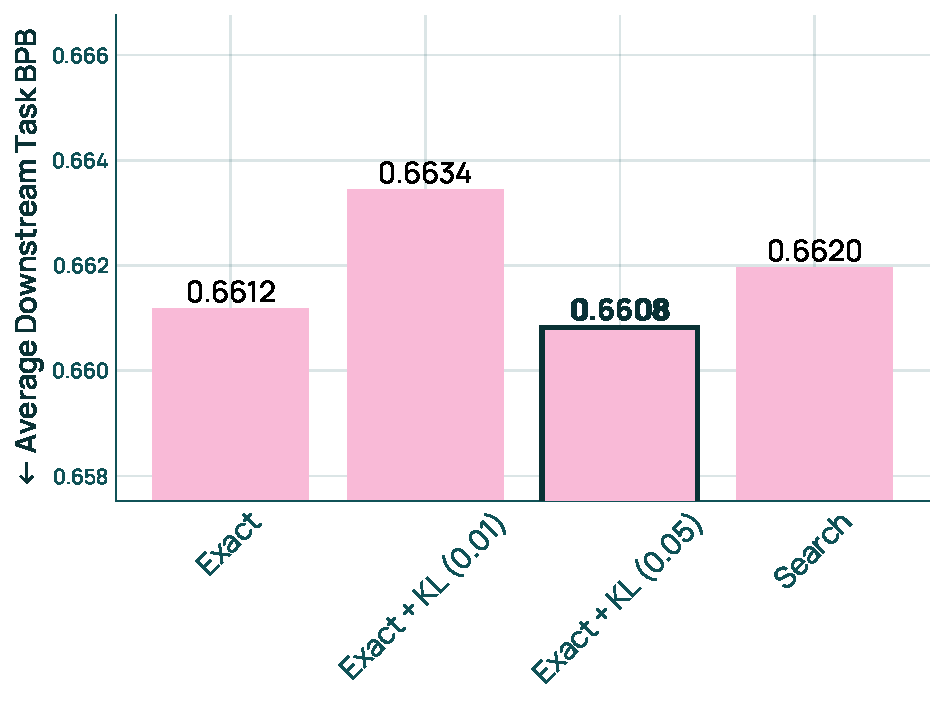
\includegraphics[width=0.49\linewidth]{figs/contribution_1/performance_solvers_olmo3.pdf}
    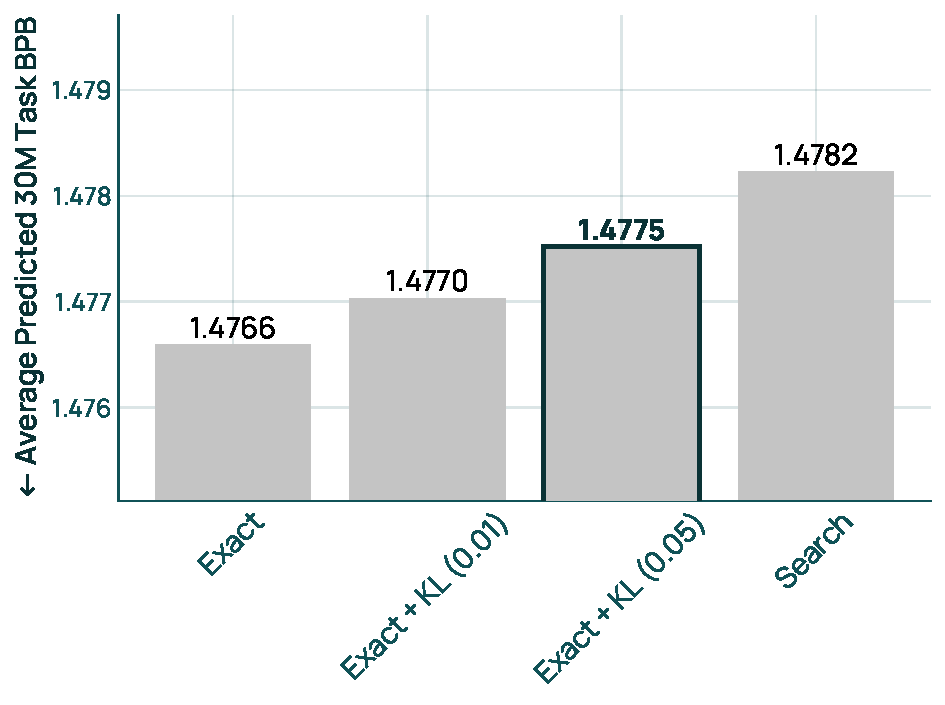
\includegraphics[width=0.5\linewidth]{figs/contribution_1/predicted_performance_solvers_olmo3.pdf}
    \caption{Performance (left) and regression fit (right) across optimization solvers when mixing across sources. The predicted performances of various solvers confirms that the exact solver minimizes the predicted BPB, as expected, followed by KL penalties of $0.01$ and $0.05$. However, the exact solver does not obtain the best downstream performance, and instead some KL regularization helps.}
    \label{fig:solvers_olmo3}
\end{figure}

\textbf{Details.} For the search approach, we used the adaptive search proposed in~\citet{wettig2025organizewebconstructingdomains}, which proceeds in multiple rounds such that the best mix from the current round is used as a Dirichlet prior to generate candidate mixes for the next round. 




